\documentclass[11pt,letterpaper,boxed]{hmcpset}
\usepackage{fullpage}
\setlength{\parskip}{6pt}
\setlength{\parindent}{0pt}
\usepackage[margin=1in]{geometry}
\usepackage{graphicx}
\usepackage{enumerate}
\usepackage{marvosym}
\usepackage{amssymb}
\usepackage{wasysym}
\usepackage{gensymb}
\usepackage{mathrsfs}
\usepackage{scrextend}
\usepackage{mathtools}
\usepackage{pgfplots}
\usepackage{xspace}
\usepackage[colorlinks]{hyperref}

\makeatletter
\renewcommand*\env@matrix[1][*\c@MaxMatrixCols c]{%
   \hskip -\arraycolsep
   \let\@ifnextchar\new@ifnextchar
   \array{#1}}
\makeatother

% --- style --- %
\renewcommand{\labelenumi}{{ (\alph{enumi})}}
\newcommand{\sand}{\quad \mbox{ and } \quad}
%\newcommand{\ds}{\displaystyle}
\allowdisplaybreaks

% --- making \xi look less awful --- %
\DeclareSymbolFont{CMletters}{OML}{cmm}{m}{it}
\DeclareMathSymbol{\xi}{\mathord}{CMletters}{"18}

% --- math --- %
\newcommand{\Z}{\mathbb{Z}}
\newcommand{\R}{\mathbb{R}}
\newcommand{\C}{\mathbb{C}}
\newcommand{\Q}{\mathbb{Q}}


\newcommand{\Lt}[1]{\mathcal{L}\crb{#1}}
\newcommand{\ilt}[1]{\mathcal{L}^{-1}\crb{#1}}

\newcommand{\pn}[1]{\left( #1 \right)}
\newcommand{\sqb}[1]{\left[ #1 \right]}
\newcommand{\crb}[1]{\left\{ #1 \right\}}
\newcommand{\lra}[1]{\left\langle #1 \right\rangle}
\newcommand{\magn}[1]{\left\lVert #1 \right\rVert}

\newcommand{\pdr}[2]{\frac{\partial #1}{\partial #2}}
\newcommand{\im}[1]{\text{im}\pn{#1}}
\newcommand{\m}[1]{\Z/#1\Z}

\newcommand{\VEC}[1]{\ensuremath{\mathbf{#1}}\xspace}
\DeclareMathOperator{\proj}{proj}
\newcommand{\vectorproj}[2][]{\proj_{\VEC{#1}}\VEC{#2}}

\newenvironment{amatrix}[1]{%
  \left(\begin{array}{@{}*{#1}{c}|c@{}}
}{%
  \end{array}\right)
}

\makeatletter
\renewcommand*\env@matrix[1][*\c@MaxMatrixCols c]{%
  \hskip -\arraycolsep
  \let\@ifnextchar\new@ifnextchar
  \array{#1}}
\makeatother

\newcommand{\spn}[1]{\text{span}\pn{#1}}

\newcommand*\Heq{\ensuremath{\overset{\kern2pt H}{=}}}

\name{Box \#$\rule{1cm}{0.15mm}$}
\class{Math 60 Section 1}
\assignment{Homework 9}
\duedate{25 May 2018}

\begin{document}

%\begin{center}
\noindent\textbf{Collaborators:} 
%\end{center} 

%\problemlist{}

\begin{problem}[Colley 5.4 \#4]
Find the value of 
\[
	\int\int\int_W z\,dV,
\]
 where $W = [-1,2]\times[2,5]\times[-3,3]$, without resorting to explicit calculation.
\end{problem}

\begin{solution}
\vfill
\end{solution}
\newpage

\begin{problem}[Colley 5.4 \#5]
Evaluate
\[
	\int_{-1}^2\int_{1}^{z^2}\int_0^{y+z}3yz^2\,dx\,dy\,dz.
\]
\end{problem}

\begin{solution}
\vfill
\end{solution}
\newpage

\begin{problem}[Colley 5.4 \#18	]
Integrate
\[
	f(x,y,z) = z
\]
over $W$, where $W$ is the region bounded by $z=0$, $x^2+4y^2=4$, and $z=x+2$.
\end{problem}

\begin{solution}
\vfill
\end{solution}
\newpage

\begin{problem}[Colley 5.4 \#29(a),(b)]
Consider the iterated integral
\[
	\int_{-2}^2\int_0^{\frac{1}{2}\sqrt{4-x^2}}\int_{x^2+3y^2}^{4-y^2}(x^3+y^3)\,dz\,dy\,dx.
\]
\begin{enumerate}
\item This integral is equal to a triple integral over a solid region $W$ in $\R^3$. Describe $W$.
\item Set up an equivalent iterated integral by integrating first with respect to $z$, then with respect to $x$, then with
respect to $y$. Do not evaluate your answer.
\end{enumerate}
\end{problem}

\begin{solution}
\vfill
\end{solution}
\newpage

\begin{problem}[Colley 5.5 \#25]
Evaluate
\[
	\int\int_D \cos(x^2+y^2)\,dA,
\]
where $D$ is the shaded region in the following figure.
\begin{center}
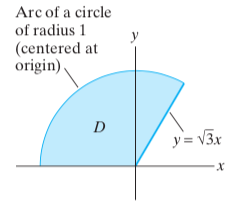
\includegraphics[scale=0.6]{circ.png}
\end{center}
\end{problem}

\begin{solution}
\vfill
\end{solution}
\newpage

\begin{problem}[Colley 5.5 \#31]
Determine
\[
	\int\int\int_W(x^2+y^2+2z^2)\,dV,
\]
where $W$ is the solid cylinder defined by the inequalities $x^2+y^2\leq 4$, $-1\leq z\leq2.$
\end{problem}

\begin{solution}
\vfill
\end{solution}
\newpage

\begin{problem}[Colley 5.5 \#34]
Determine the value of
\[
	\int\int\int_W \frac{dV}{\sqrt{x^2+y^2+z^2}},
\]
where $W$ is the region bounded by the two spheres $x^2+y^2+z^2=a^2$ and $x^2+y^2+z^2=b^2$, for $0<a<b.$
\end{problem}

\begin{solution}
\vfill
\end{solution}
\newpage

\begin{problem}[Colley 5.5 \#38]
Determine
\[
	\int\int\int_W(2+\sqrt{x^2+y^2})\,dV,
\]
where $W = \crb{(x,y,z) | \sqrt{x^2+y^2}\leq z/2 \leq 3}.$
\end{problem}

\begin{solution}
\vfill
\end{solution}

\end{document}